\chapter{Ferramentas de Análise Estática de Código Fonte}\label{chap:ferramentas}

A realização da análise estática de código fonte de maneira manual, ou seja, sem
o auxílio de uma ferramenta que automatize esse processo, é bastante custosa e
praticamente impraticável, já que seria necessário um especialista passar em
cada arquivo fonte realizando as análises necessárias. Sendo assim, seria
praticamente impossível a inserção dessa prática no ciclo de desenvolvimento de
qualquer software, tendo em vista que o custo seria gigantesco, salvo alguns
casos específicos onde esse tipo de atividade se faz necessária. Com isso em
mente, as ferramentas de análise estática de código fonte são essenciais para
que se torne viável a utilização da mesma no desenvolvimento de software.

Visando automatizar o processo de análise estática, as ferramentas varrem
arquivos e diretórios em busca do código fonte, analisam-os e apresentam
métricas para o usuário, de maneira quantitatica ou qualitativa. Muitas dessas
ferramentas são bem complexas e para realizar esse processo de análise do
código fonte realizam várias etapas intermediárias. Entretanto, existem
ferramentas que visam analisar o código fonte de maneira mais simples, menos
complexa, onde será menos custoso computacionalmente, para que possa dar uma
resposta mais rápida para o usuário.

As ferramentas de análise estática de código fonte, em geral, se assemelham
bastante com a estrutura de um compilador, onde se faz uma análise do código
fonte, se controi um modelo/estrutura desse código, realiza uma análise sobre
essa estrutura e apresenta os resultados para o usuário. Segundo
\citeonline{chess&west2007}, os problemas enfrentados por grande parte das
ferramentas de análise estática de código fonte se assemelham aos enfrentados na
contrução de compiladores e na otimização dos mesmos. Tendo em vista que este
trabalho tem um foco em segurança de código fonte, na Seção
\ref{sec:ferramentasseguranca} é apresentada a estrutura da maioria das
ferramentas que realizam análise estática voltada para a segurança do código
fonte.


\section{Ferramentas de Análise Estática de Segurança de Código Fonte}
\label{sec:ferramentasseguranca}

Para se entender o funcionamento de uma ferramenta de análise estática de
segurança de código fonte genérica é apresentado um diagrama de blocos na Figura
\ref{fig:diagrama_ferramenta_seguranca}, onde \citeonline{chess&west2007}
resumem essa sistemática.

\begin{figure}[h]
  \centering
  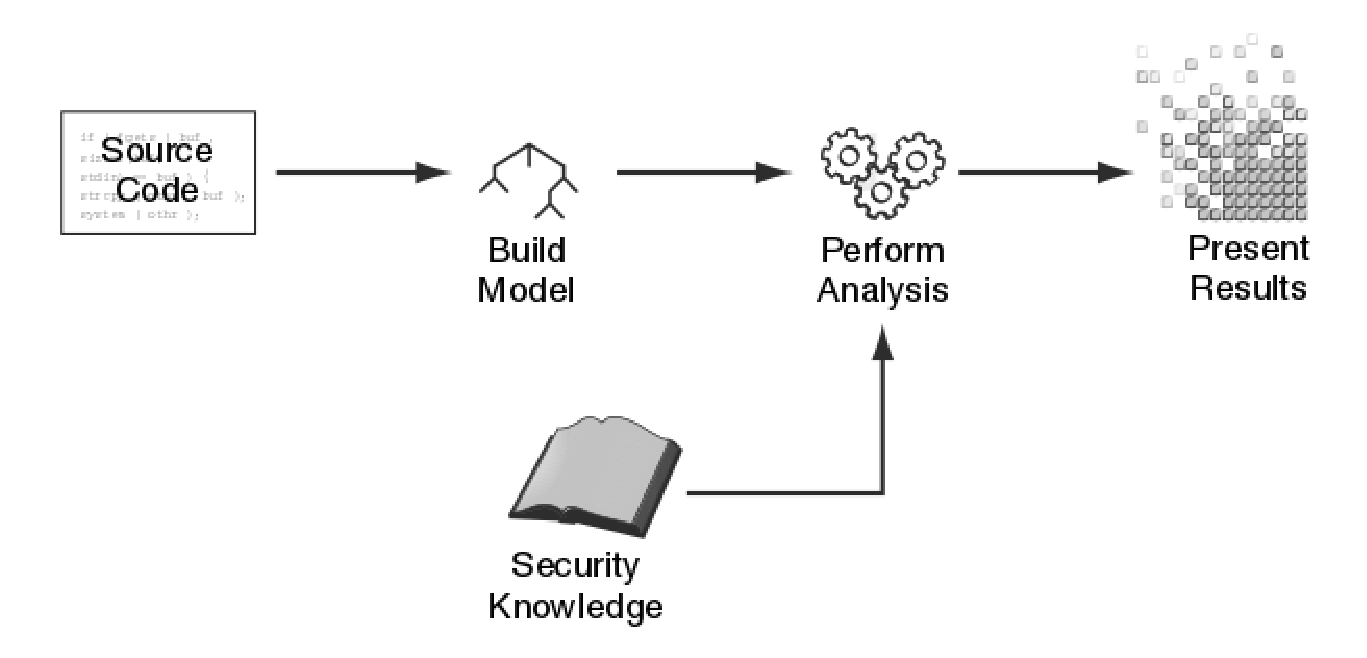
\includegraphics[width=0.8\textwidth]
      {figuras/diagrama_ferramenta_seguranca}
      \caption{Diagrama de blocos de uma ferramenta genérica \cite{chess&west2007}}
  \label{fig:diagrama_ferramenta_seguranca}
\end{figure}

Como apresentado na Figura \ref{fig:diagrama_ferramenta_seguranca}, essas
ferramentas possuem um código fonte como entrada, constroem um modelo baseado
nesse código fonte, realizam uma análise nesse modelo construído baseado em um
conhecimento prévio em segurança de código e finalmente apresentam os resultados
para o usuário. Esse fluxo é similar ao que foi apresentado no início deste
capítulo, logo, o funcionamento das ferramentas de análise de código fonte em
geral seguem a mesma estrutura, simplesmente, alterando a forma que é realizada
a análise em si, onde vai variar dependendo do objetivo da análise estática.

Nas seções a seguir serão apresentados em mais detalhes cada um dos blocos
representados na Figura \ref{fig:diagrama_ferramenta_seguranca}.


\subsection{Construção do Modelo}

A fase de construção de um modelos baseado no código fonte de entrada é
praticamente identica ao que é realizado por um compilador. São elaboradas as
seguintes atividades sequencialmente:

\begin{itemize}
\item Análise léxica
\item \textit{Parsing} ou Análise sintática
\item Análise semântica
\end{itemize}

Na análise léxica, todo o código fonte é transformado em uma série de
\textit{tokens}, descartando partes não importantes do código, como espaços em
branco e comentários \cite{chess&west2007}. Existem algumas ferramentas, como o
\textit{Flex}\footnote{\url{http://flex.sourceforge.net/}}, que auxiliam nessa
tranformação do código fonte em \textit{tokens}, sendo essa bastante utilizada
na construção de compiladores. Para a execução dessa atividade utiliza-se
bastante de técnicas como expressões regulares para a identificação dos
\textit{tokens} desejados. O Código \ref{flex} exemplifica como pode ser feita uma
análise ĺéxica bastante simples com a ferramenta \textit{Flex}.

\begin{lstlisting}[caption={Análise léxica simples com a ferramenta \textit{Flex}}, label=flex]
  [ \t\n]+          { //ignorando espaços em branco }
  \/\/.*            { //ignorando comentários }
  if                { return IF; }
  for               { return FOR; }
  (                 { return LEFT_PARETHESIS; }
  )                 { return RIGHT_PARENTHESIS; }
\end{lstlisting}

Na fase de \textit{parsing} ou análise sintática, o \textit{stream} de
\textit{tokens} recebidos da análise léxica é manipulado tentando enquadrá-lo a
gramática de contexto livre (\textit{context free-grammar} ou simplesmente
\textit{CFG}) que é definida. A gramática de contexto livre nada mais é do que
um conjunto de \textit{production} (regras) que descrevem os símbolos daquela
linguagem \cite{chess&west2007}. A ferramenta
\textit{GNU Bison}\footnote{\url{https://www.gnu.org/software/bison/}} é
bastante utilizada para a definição dessa gramática de contexto livre, sendo
essa facilmente integrada com o \textit{Flex}. O Código \ref{bison} exemplifica
a definição de uma gramática de contexto livre simples.

\begin{lstlisting}[caption={Definição de uma \textit{CFG} simples com a ferramenta
\textit{GNU Bison}}, label=bison]
  entrada    
          : /* vazio */
          | entrada linha
          ;
  linha     
          : '\n'
          | expressao '\n'
          ;
  expressao
          : IF LEFT_PARENTHESIS expressao RIGHT_PARENTHESIS bloco
          ;
\end{lstlisting}

Com esse tipo de definição de gramática de contexto livre e o \textit{stream}
de \textit{tokens} pode-se chegar a uma \textit{Parse Tree}, onde facilita a
visualização da estrutura do código, como pode ser visto na Figura
\ref{fig:parse_tree} apresentada por \citeonline{chess&west2007}.

\begin{figure}[h]
  \centering
  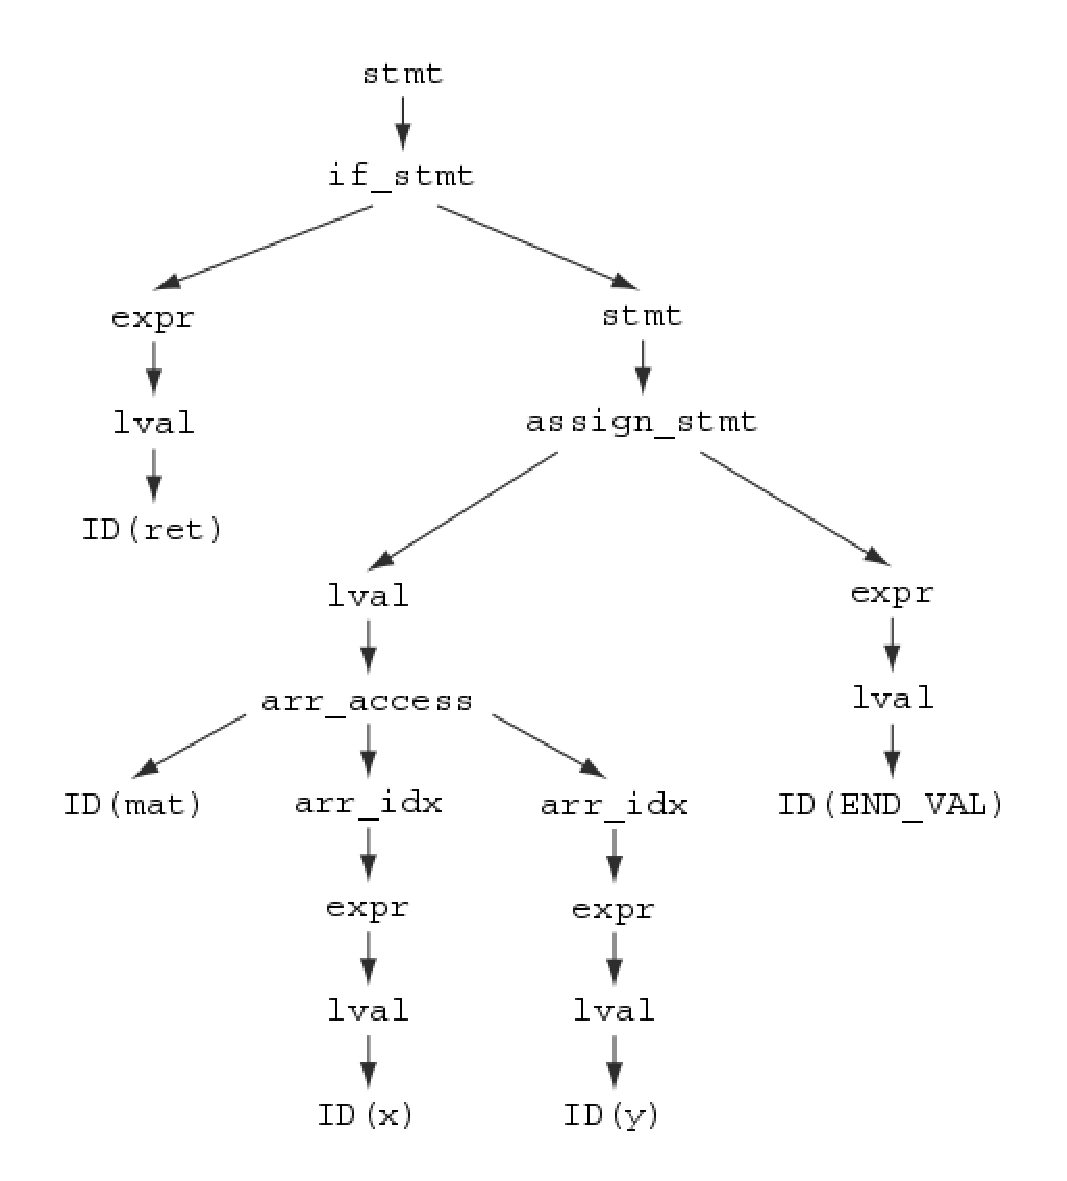
\includegraphics[width=0.6\textwidth]
      {figuras/parse_tree}
      \caption{Exemplo de \textit{Parse Tree} \cite{chess&west2007}}
  \label{fig:parse_tree}
\end{figure}

Muitas ferramentas de análise estática de segurança de código fonte realizam as
suas análises diretamente na sua \textit{Parse Tree} já que essa está bem
próximo ao código que foi escrito, mas para realizar análises mais complexas
pode ser inconveniente, sendo necessário o desenvolvimento de uma
\textit{Abstract Syntax Tree} (\textit{AST}) \cite{chess&west2007}. Na
\textit{AST} vários detelhes relacionado a gramática são abstraídos a fim de
facilitar a análise da mesma, a Figura \ref{fig:ast} nos mostra um exemplo dessa
estrutura de dados.

\begin{figure}[h]
  \centering
  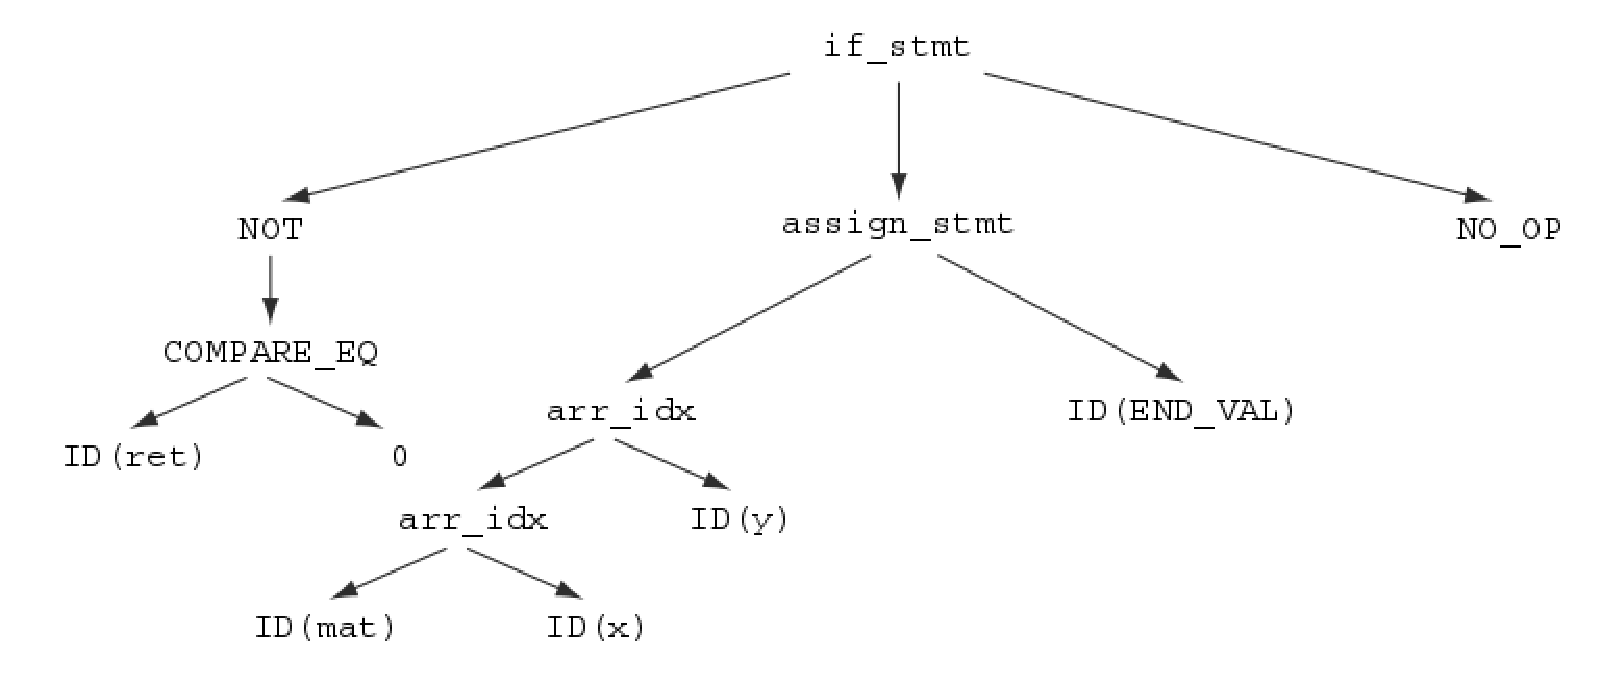
\includegraphics[width=1.0\textwidth]
      {figuras/ast}
      \caption{Exemplo de \textit{AST} \cite{chess&west2007}}
  \label{fig:ast}
\end{figure}

Em paralelo a construção dessas estruturas de dados a ferramenta de análise
estática constroi também a chamada tabela de símbolos, onde nela são associados
os identificadores, os seus respectivos tipos e um ponteiro para onde os mesmos
foram declarados ou definidos \cite{chess&west2007}. Com isso feito, as
ferramentas realizam uma análise semântica do código, como por exemplo
\textit{type checking}. É após a análise semântica que as ferramentas de análise
estática e os compiladores começam a se diferenciar.

Para algumas ferramentas de análise estática são necessárias algumas formas de
representação intermediária do código, como gráficos de fluxo do programa, fluxo
dos dados do programa e chamadas de métodos ou funções. Dependo do que a
ferramenta se propõe a fazer, a elaboração desse tipo de representação é
essencial.

\subsection{Realização da Análise}

Após a contrução do modelo apresentada anteriormente, inicia-se a fase de
análise desse modelo, que como foi dito no início desta seção depende de
conhecimentos relacionado a segurança de código fonte. Devido a essa análise ser
diferente dependendo do objetivo da ferramenta e o intuito deste capítulo é
apenas uma visão geral do funcionamento das mesmas, não foi aprofundado esse
assunto, apenas serão apresentados os diferentes tipos de análise que podem ser
realizadas.

Existem basicamente dois tipos de análise que podem ser realiadas, sendo elas
análise intraprocedural (local) ou interprocedural (global). Como o próprio nome
já diz, a análise intraprocedural ou local é a análise realizada apenas no contexto
daquele procedimento ou função, ou seja, não será levado em considerção nada que
não esteja presente naquele contexto, por exemplo, chamadas a outras funções
dentro da função analisada serão desconsideradas. A análise interprocedural ou
global leva em consideração a interação entre as funções, sendo essa mais
completa, entretanto, bem mais complexa. Algumas ferramentas utilizam a análise
local para a realização da análise global, onde a análise local gera um sumário
de todas as funções e durante a análise global esse sumário é consultado,
facilitando o processo.

Segundo \citeonline{chess&west2007}, a flexibilidade das ferramentas para a
definição de regras para a realização da análise do código fonte é essencial
para que o usuário tenha o controle e a liberdade para definir seu próprio
processo de análise quando for necessário.

\subsection{Apresentação dos Resultados}

Com a realização da análise do código fonte concluída os resultados devem ser
aresentados para o usuário de maneira adequada para que o mesmo possa conseguir
utilizar aquela informação para a tomada de alguma decisão. Em geral,
ferramentas que desejam chegar ao mercado, e não apenas o público acadêmico, devem
permitir que os usuários agrupem e ordenem os resultados, eliminem resultados
indesejados e a ferramenta deve explicar a significância dos resultados
\cite{chess&west2007}.

As ferramentas mais utilizadas no mercado para a realização de análise estática
de segurança de código fonte são integradas a alguma \textit{IDE}
(\textit{Integrated Development Environment}), o que facilita para o
desenvolvedor utiliza-la, sendo os \textit{reports} das ferramentas apresentados
na maioria das vezes diretamente no código e sendo autoexplicativos, inclusive
apresentando métodos para a validação da possível vulnerabilidade e qual seria
uma possível correção.


\subsection{Classificação das Ferramentas}\label{sec:classificacaoferramentas}

Além de entender sobre o funcionamento das ferramentas de análise estática de
segurança de código fonte, é importante saber como as mesmas são classificadas.
Segundo \citeonline{paul:2001}, as ferramentas podem ser classificadas baseado
em como elas realizam as suas análises, podendo ser uma análise \textit{sound},
heurística ou completa.

Uma ferramenta classificada como \textit{sound} ela é 100\% correta em todos os
seus julgamentos \cite{paul:2001}, ou seja, todas as ameaças de vulnerabilidades que a
ferramenta aponta realmente são vulnerabilidades. Isso não quer dizer que esse
tipo de ferramenta é a ferramenta ideal, pois sempre garantir que o que ela está
dizendo é verdade não assegura que todas as vulnerabilidades do código foram
encontradas. A principal característica desse tipo de ferramenta é a baixa taxa
de falsos positivos, entretanto, a taxa de falsos negativos pode ser grande, que
seria o caso de haver vulnerabilidade no código fonte e a mesma não indicar-la.

Agora quando a análise é feita baseada nas regras que podem ser automaticamente
derivadas do código através de \textit{machine learning} do código existente a
ferramenta é classificada como heurística \cite{paul:2001}. Por exemplo, quando
se encontra uma função \textit{open()} durante a análise do código, espera-se
que exista em alguma lugar uma função \textit{close()}, esse tipo de análise
pode trazer vários falsos positivos, assim como falsos negativos.

Tendo em vista esses dois tipos de análise, o ideal seria a união dos dois tipos
de análise apresentadas, as ferramentas que tentam implementar isso são chamadas
de ferramentas completas. Esses ferramentas geralmente possuem resultados bem
melhores do que ferramentas apenas heurísticas ou \textit{sound}, e se utilizam
de técnicas já mencionadas neste capítulo como acompanhamento do fluxo de dados
e controle de fluxo de execução \cite{paul:2001}.

Na seção \ref{metodologia:testehipoteses} foram análisadas algumas ferramentas
de análise estática de código fonte, sendo selecionada a ferramenta
\textit{Cppcheck}, que apesar de tentar se apresentar como uma ferramenta
\textit{sound} foi a que melhor se adaptou ao contexto da pesquisa. Em situações
reais percebe-se que o desenvolvimento de uma ferramenta completa é algo ainda a
ser melhor trabalho, ainda se apresentando como uma referência de ferramenta
ideal e não algo palpável.
